\section{History based security specifications}
\label{sec:history_def}
Our approach must specifically be able to encode and evaluate \emph{dynamically} changing privacy constraints on a certain subset of relevant information. Additionally, these pieces of information are also dynamic and constantly changing while our system under test is actively operating. This poses several challenges in regards to how we can specify these constraints over the whole body of information beforehand. 
Instead, we have decided to utilise a \emph{history} based encoding scheme that takes into account the sequential nature of privacy changes over several time steps.
\subsection{What constitutes a history}
We rely on a central data structure, a sequential \emph{history} of abstract events, that each encodes a high-level operation depending on the system under test.
Formally, we can thus define any history \(h\) as
\[
    h_n = \{ev_1,ev_2,\dots, ev_n\},
\]
where \(n\) denotes the size of the given history and any \(ev_i\) represents the \(i\)-th operation or \emph{event} in the history.
Given that the history itself is in no way responsible for the way in which it is interpreted, we impose no requirements on the internal structure of the event type.
\subsection{Generating histories for Hagrid}
Given our general definition of a history, we can now look at the content of histories that we use to test our model of HAGRID. 
As described in chapter \ref{sec:hagrid_structure}, we want to be able to describe the process of verifying a given subset of valid identities belonging to a PGP key and similarly revoking these identities in a similar fashion. Note that these two operations, \emph{verifying} and \emph{revoking} identities are the central operations, that drive the dynamic declassification and reclassification of private data in our server.
We therefore define 3 abstract types of events, that can be included in a history: 
\begin{enumerate}
    \item \emph{Upload(k)} -- Given some key \(k\), this event describes the action of adding a fresh PGP key to the internal state of our server.
    \item \emph{Verify(ids,fingerprint)} -- Given a set of identities, this event describes the action of \emph{declassifying} these formerly private identities, given that they belong to the key identified by the corresponding \emph{fingerprint}.
    \item \emph{Revoke(ids, fingerprint)} -- Given a set of identities, this event describes the action of \emph{reclassifying} these formerly public identities, given that they belong to the key identified by the corresponding \emph{fingerprint}.
\end{enumerate}

\subsection{How to evaluate histories}
Given a history of some arbitrary size, we now require a method of inspecting the sequence of events and compute the \emph{effect} that each event in the history has on the privacy state space of our server. 
Specifically, our goal is to run a symbolic execution of a history, which ultimately computes the totality of valid visibility associations between keys and their identities. Note that this symbolic history execution doesn't have to match the actual execution process, because we can omit the server model as our middle man and compute the privacy state for all keys directly.

\paragraph{A formal description of history evaluation}
\label{sec:history_def}

Evaluation of arbitrary histories can be formally approximated by a set of state machines \(S_i\). Each state machine tracks the visibility state of its associated identity \(i\).

To show how this formalization works, let us first look at a simpler case where we only consider histories of events that affect a single key with only one associated identity. 

We can then define a state machine \(S\) which is a quintuple \((\Sigma,Q,s_0,\delta,F)\), where:
\begin{itemize}
    \item \(\Sigma\) is the input alphabet given by the set \(\{\text{Upload},\text{Verify},\text{Revoke}\}\), corresponding to our history event types.
    \item \(Q\) is the finite set of states \(\{\Theta,U,C,R\}\).
    \item \(s_0\) is the initial state of any identity, denoted as \(S_0\).
    \item \(\delta\) is the state transition function, defined by the following state transitions:
    \begin{equation}
        \begin{aligned}
            &\Theta \xrightarrow{\text{Upload}}U \\
            &U \xrightarrow{\text{Verify}}C \\
            &C \xrightarrow{\text{Revoke}}R \\
            &R \xrightarrow{\text{Verify}}C
        \end{aligned}
    \end{equation}
    \item F is the empty set of final states.
\end{itemize}

The states of this state machine represent the privacy state after each transition, where a transition to \(U\) means that the given identity has been uploaded, yet remains undiscoverable until further state changes. The \(C\) state occurs when the given identity gets verified and therefore publicly available, whereas the \(R\) state describes the exact opposite, the given identity is private and must therefore first be re-verified to become available again.
\\

We can now generalize this state machine to support histories containing arbitrary amounts of keys and identities. Let's consider the set of state machines \(\{S_{i,k}\}\), where all state machines share their set of states and initial state with \(S\). 

Given some event \(E_{i,k}\) and some state \(s \in Q\), we define \( \exists {s'} \subseteq \delta_{i',k'}(E_{i',k'},s) \) if, and only if \( \exists S_{i',k'} .\, i' = i \wedge k' = k\).
Furthermore, it is easy to see that any event \(E(t,f)\), where \(t\) is a set of identities can also be denoted as the set \(E' = \{E_{t_i,f} | t_i \in t\} \). That means, that any event that affects multiple identities at once can be equivalently formulated as a sequence of the same event that each affects a single event from the original set.
For the sake of consistency, we will use \(\text{Upload}_{i,k}\), even though the \mintinline{Text}{Upload} event does not specifically contain the set of identities it affects. This means, that \mintinline{Text}{Upload(k)} is equivalent to \(\{(i,k) \; \big|\; i \in \text{k.identities}\}\).

\begin{figure}[h]
    \centering
    \begin{tikzpicture}[->,>=stealth',shorten >=1pt,auto,node distance=3.8cm,semithick]
    
        \node[initial, state] (A)                      {$S_0$};
        \node[state]          (B) [above right of=A]   {$U$};
        \node[state]          (C) [below right of=B]   {$C$};
        \node[state]          (E) [below       of=B]   {$E$};
        \node[state]          (D) [below right  of=E]  {$R$};

    
        \path   (A)     edge               node {$\text{Upload}_{i,k}$}          (B)
                        
                (B)     edge               node {$\text{Verify}_{i,k}$}          (C)
                (C)     edge [bend left]   node {$\text{Revoke}_{i,k}$}          (D)
                (D)     edge [bend left]   node[pos=0.7] {$\text{Verify}_{i,k}$}          (C)
                (B)     edge               node {$\text{Get}_{i,k}$}               (E)
                (A)     edge               node[pos=0.3] {$\text{Get}_{i,k}$}               (E)
                (D)     edge [bend left]   node[above right] {$\text{Get}_{i,k}$}               (E)
                (E)     edge [bend left]   node  {$\epsilon$}                    (A)
                        edge [bend left]   node {$\epsilon$}                    (B)
                        edge [bend right=70]  node  {$\epsilon$}                    (D);
    
    \end{tikzpicture}
    \caption{Visualization of a state machine over a history}
\end{figure}

In order to emphasize which states support a successful key request, we included an additional state \(E\), which is only reachable by transitions marked with \(\text{Get}_{i,k}\). We can think of \(E\) as a kind of implicit error state, which tells us, that the system encountered an attempt to retrieve a key \(k\), while the state machine associated with \(k\) was still in a state, that made returning a key impossible. 

This will only ever occur if the state machine is either in its initial state \(S_0\), or all state machines \(t_{k,i}\) for a given \(k\) are currently in the state \(U\).

\paragraph{Determining the final states produced by a history}
We can determine \emph{all} relevant privacy states by simply collecting the final state of each state machine after the history has been completely evaluated.
Formally, the set of all uploaded keys can be constructed from a given history as follows:
\newcommand{\pctext}[2]{\text{\parbox{#1}{\centering #2}}}
\[U = \biggl \{(i,k) \;\bigg|\; \text{Upload}_{i,k} \in H \biggr\}\]
where \(\text{Upload}_{i,k} \in H \Leftrightarrow \exists x. H_x = \text{Upload}_{i,k}\). 
We further define the total set of all revoked and verified \mintinline{Text}{(Identity,Key)} pairs as:

\begin{equation}
    \label{eq:states}
    \begin{alignedat}{2}
        C &= \biggl \{(i,k) &&\;\bigg|\; \pctext{2.4in}{\(\exists t,t'\;.\; H_t = \text{Upload}_{i,k},H_{t'} = \text{Verify}_{i,k}, t < t', \forall z > t'. H_z \neq \text{Revoke}_{i,k}\)}  \biggr \} \\[10pt]
        R &= \biggl \{(i,k) &&\;\bigg|\; \pctext{2.4in}{\(\exists t,t'\;.\; H_t = \text{Upload}_{i,k},H_{t'} = \text{Revoke}_{i,k}, t < t', \forall z > t'. H_z \neq \text{Verify}_{i,k}\)}  \biggr \}
    \end{alignedat}
\end{equation}

\(C\) therefore contains all uploaded pairs \((i,k)\) for which there exists a verification event \(\text{Verify}_{i,k}\) at some point after the upload, while all revocation events \(\text{Revoke}_{i,k}\) come \emph{before} the verification. Conversely, we invert that condition for \(R\) and require all \(\text{Verify}_{i,k}\) events to occur before the eventual revocation.


\paragraph{History evaluation against a server model}
Determining which associations between identities and keys are valid based on a history alone is only the first step of actually \emph{testing} HAGRID. To complete our history-based approach, we require a way of comparing the results of the symbolic history execution to the actual server state. Only then can we determine whether the model adheres to our chosen privacy constraint.

The solution to this requirement consists of two parts in total. As a first step, we need to \emph{execute} the history on a given server backend. In a second step, we can then collect all available data from the server and compare the results to our previously computed visibilities. 
\\ \\
In order to visualize the execution of a history, we can look at the following example: 
\begin{figure}[H]
    \label{fig:history}
    \centering
    \makebox[\textwidth][c]{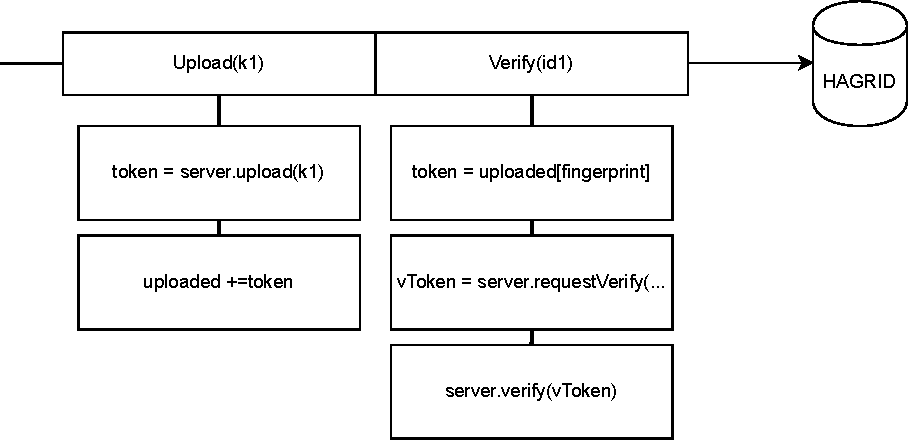
\includegraphics[width=1.1\textwidth]{images/history_small.pdf}}%
    \caption{An example of a history execution}
\end{figure}

Notice how \mintinline{Text}{Verify} abstracts over the two separate steps of \emph{requesting} a verification and the subsequent actual verification step. \\ \\
Executing the history is crucial because a mere evaluation of the history alone doesn't tell us anything about how the server actually behaves. Instead, we want to \emph{compare} the result of our own history evaluation against the server responses.



\paragraph{Determining invalid associations}
\label{sec:priv_condition}
Given that we now have an abstract model to evaluate the valid associations of keys and identities based on a history of events, we can now determine whether some HAGRID backend adheres to its privacy model. This is done by computing the \emph{difference} between the states that were determined to be visible by our history run and those returned by the backend.

For this purpose, we further abstract over the sets \(U,C\) and \(R\) by introducing the sets \(\text{Public},\text{Private}\) and \(\text{Revoked}\),
each directly representing the privacy state of their elements: 
\begin{align}
    \text{Public}  &= \bigl \{ (i,k) \; \big|\; (i,k) \in C\bigr\}  \nonumber \\
    \text{Private} &= \bigl \{ (i,k) \; \big|\; (i,k) \in U \wedge (i,k) \notin C \wedge (i,k) \notin R\bigr\}  \\
    \text{Revoked} &= \bigl \{ (i,k) \; \big|\; (i,k) \in R\bigr\} \nonumber
\end{align}

It should be noted that including a specific case for revoked identities would not be strictly necessary, as HAGRID returns an empty response both in the instance of \mintinline{Text}{Private} and \mintinline{Text}{Revoked} identities, rendering a distinction between these two states impossible from the outside. For the sake of accuracy, we still chose to include a \mintinline{Text}{Revoked} category, because it can convey useful information in the hypothetical scenario where HAGRID \emph{does} return a non-empty response and we want to include the exact kind of mismatch in an error message.

We can now use these three sets \(\text{Public},\text{Private}\) and \(\text{Revoked}\) and determine the set of \(\text{Valid}\) and \(\text{Invalid}\) associations between keys and identities. This is done by retrieving all accessible information from the abstract server model and comparing each entry to the computed privacy state as shown in \ref{eq:states}. Let \(S\) be the set of all \mintinline{Text}{(Identity,Key)} pairs, representing the total retrieved state of our abstract server model. We can then define \(\text{Valid}\) as follows:  

\begin{equation}
    \text{Valid} = \biggl \{ (i,k) \;\bigg|\; \pctext{1.97in}{
        \( ((i,k) \in \text{Public}  \wedge (i,k) \in S)\; \vee \; \)
        \( ((i,k) \in \text{Revoked} \wedge (i,k) \notin S)\; \vee \; \)
        \( ((i,k) \in \text{Private} \wedge (i,k) \notin S) \) }  
    \biggr \}
\end{equation}
That is, for a given \mintinline{Text}{(Identity, Key)} pair to be considered valid, it must satisfy one of three conditions: 
\begin{enumerate}
    \item The pair \((i,k)\) is a confirmed association and is also included in the retrieved server state \(S\)
    \item The pair \((i,k)\) is a revoked association and is missing from the retrieved server state \(S\)
    \item The pair \((i,k)\) is neither revoked nor confirmed (but has been uploaded to the server) and is missing from the retrieved server state
\end{enumerate}
Conversely, the definition of \(\text{Invalid}\) can be denoted as: 
\begin{equation}
    \text{Invalid} = \biggl \{
        (i,k) \;\bigg|\; \pctext{1.97in}{
            \((i,k) \in \text{Public}  \wedge (i,k) \notin S \; \vee \)
            \((i,k) \in \text{Revoked} \wedge (i,k) \in S \; \vee \)
            \((i,k) \in \text{Private} \wedge (i,k) \in S\)
        }
    \biggr \}
\end{equation}
Again, for a given \mintinline{Text}{(Identity,Key)} pair to be considered invalid, it must satisfy one of three conditions:

\begin{enumerate}
    \item The pair \((i,k)\) is a confirmed association but has no respective entry in the retrieved server state \(S\)
    \item The pair \((i,k)\) is a revoked association but is still present in the retrieved server state \(S\)
    \item The pair retrieved is neither confirmed nor revoked (but has been uploaded to the server) but is still present in the retrieved server state
\end{enumerate}

Based on these two partitions of identities and key, we can now define a general constraint that determines whether the Hagrid server model only performs valid declassifications (and reclassifications). 
Let \(H\) denote the set of all histories considered by a specific test instance. Let \(\text{Invalid}_h\) denote the set of invalid associations computed from some history \(h \in H\). We can then express that a model of Hagrid is safe, if and only if the set of invalid associations is empty for all histories that were taken into account:
\[
    \forall h \in H \; .\; \text{Invalid}_h = \emptyset
\]

\paragraph{Testing both functional correctness and privacy constraints at the same time}
During a presentation of our preliminary progress on the VerifyThis2020 challenge earlier this year in April, a member of one of the participating teams raised the question of how our approach handles a theoretically maximally secure HAGRID server, that never returns any key data of any kind. Such a system would achieve the highest possible protection of PGP keys because its behaviour would prevent it from ever leaking any information, private or otherwise. On the other hand, this behaviour would simultaneously render the server completely useless at its intended usage as a public PGP key server.

Given our formal approach of verifying privacy constraints as outlined in this chapter, we can strictly enforce the privacy of \emph{unverified} identities, while simultaneously ensuring that the server correctly returns declassified data in all other cases, where the release of that information is actually permissible. 

\paragraph{Reformulating the example runs from chapter \ref{ref:Declass_and_Inter} using state machines}
Looking at our previous history examples from chapter \ref{ref:Declass_and_Inter} we can see quite clearly, that our encoding of histories in terms of state machines gives us a surprisingly natural representation of our privacy states at every intermediate step of our history.
Let \(h_1=\{Upload(k1),Get(id1),Upload(k2)\}\) and \(h_2 = \{Upload(k1),Get(id1),Upload(k2),Verify(id1),Get(id1)\}\).

We can now visualize both history runs accordingly, by showing the respective state transitions of their state machines at each step:

\begin{figure}[H]
    \begin{minipage}[t]{0.5\textwidth}
        \centering
        \begin{tikzpicture}[->,>=stealth',shorten >=1pt,auto,node distance=1.5cm,semithick]
            \node[initial, state]   (A)                         {$S_0$};
            \node[state]            (B) [below of=A]            {$U$};
            \node[state]            (E) [below of=B]            {$E$};
            
            \path   (A) edge    node    {$\text{Upload}_{id1,k1}$}  (B)
                    (B) edge    node    {$\text{Get}_{id1,k1}$}     (E);
        \end{tikzpicture}
        \caption*{State flow of \{\mintinline{Text}{Upload(k1),Get(id1)}\}}
    \end{minipage}
    \begin{minipage}[t]{0.5\textwidth}
        \centering
        \begin{tikzpicture}[->,>=stealth',shorten >=1pt,auto,node distance=1.5cm,semithick]
            \node[initial, state]   (A)                         {$S_0$};
            \node[state]            (B) [below of=A]            {$U$};

            \path   (A) edge    node    {$\text{Upload}_{id2,k2}$}  (B);
        \end{tikzpicture}
        \caption*{State flow of \{\mintinline{Text}{Upload(k2)}\}}
    \end{minipage}
    \caption{State flow of \(h_{1}\) split up into two separate state machines }
\end{figure}
From this, we can easily determine that our set of publicly accessible information is empty for history $h_1$. Looking at the following state transition graphs for $h_2$ we can also see quite clearly how adding an instruction like \mintinline{Text}{Verify(id1)} changes that:
\begin{figure}[H]
    \begin{minipage}[t]{0.5\textwidth}
        \centering
        \begin{tikzpicture}[->,>=stealth',shorten >=1pt,auto,node distance=1.5cm,semithick]
            \node[initial, state]   (A)                         {$S_0$};
            \node[state]            (B) [below of=A]            {$U$};
            \node[state]            (C) [below of=E]            {$C$};
            \node[state]            (E) [below of=B]            {$E$};
            \node[state]            (V) [below of=C]            {$\epsilon$};
            
            \path   (A) edge    node    {$\text{Upload}_{id1,k1}$}  (B)
                    (B) edge    node    {$\text{Get}_{id1,k1}$}     (E)
                    (E) edge    node    {$\text{Verify}_{id1,k1}$}  (C)
                    (C) edge    node    {$\text{Get}_{id1,k1}$}     (V);
        \end{tikzpicture}
        \caption*{State flow of \{\mintinline{Text}{Upload(k1),Get(id1),} \mintinline{Text}{Verify(id1),Get(id1)}\}}
    \end{minipage}
    \begin{minipage}[t]{0.5\textwidth}
        \centering
        \begin{tikzpicture}[->,>=stealth',shorten >=1pt,auto,node distance=1.5cm,semithick]
            \node[initial, state]   (A)                         {$S_0$};
            \node[state]            (B) [below of=A]            {$U$};

            \path   (A) edge    node    {$\text{Upload}_{id2,k2}$}  (B);
        \end{tikzpicture}
        \caption*{State flow of \{\mintinline{Text}{Upload(k2)}\}}
    \end{minipage}
    \caption{State flow of \(h_{2}\) split up into two separate state machines }
\end{figure}

As \(h_2\) contains a sound \{\mintinline{Text}{Upload(...),Verify(...)}\} sequence, the state machine associated with \(k_1\) and \(id_1\) ends in a state, that we have defined as belonging to a valid \emph{public} state. 